
\subsection{N-band imaging}
\label{ssec:recipes_img_n}

\subsubsection{N-band imaging flatfield}
\label{n_img_flatfield}
\label{rec:n_img_flatfield}
\label{sssec:n_img_flatfield}
\label{n_img_flat}
\label{rec:n_img_flat}
\label{sssec:n_img_flat}
\label{metis_n_img_flat}
\label{rec:metis_n_img_flat}
\label{sssec:metis_n_img_flat}

The purpose of the flat-field calibration is to determine
pixel-to-pixel gain variations and large scale illumination variations
(due to inhomogeneities of optical elements in the telescope or
instrument). Calibration frames are obtained either during day time
using the black-body lamp of the \ac{WCU} (internal flats) or by taken
images of the twilight sky (twilight flats). Advantages and
disadvantages of the two types of flat are discussed in
\cite{METIS-calibration_plan}.

MIR detectors are typically unstable in that they show gain
fluctuations on rather short time scales, hence science exposures may
have a different flat-field structure from those captured by the
calibration flats.  While the GeoSnap detector is expected to be more
stable than the AQUARIUS detector, its stability properties need to be
studied further in order to assess whether science images can be flat
fielded.  N-band flat fields will be taken in any case for quality
control and monitoring purposes.

Since the operational concept for twilight flats needs to be refined
during commissioning at the telescope, the current recipe design is
primarily valid for internal flats.

This recipe creates a master flat for the GeoSnap detector (N-band
imaging) from lamp or sky images matched by various setup parameters
as detailed below.  A set of internal flats includes a number of
exposures with \CODE{LAMP OFF}, which will be used for dark
subtraction. For twilight flats a master dark will be subtracted. The
master flat is obtained by the slope of a linear fit of the pixel
values against the illumination level of the exposures.

The quality control parameters give various statistics for each input
frame (mean, standard deviation, etc.), the standard deviation of the
normalised master flat and the number of bad pixels identified by the
recipe. If a bad-pixel map is provided on input, it is updated,
otherwise a new one is created.

\begin{recipedef}
  Name:                & \REC{metis_n_img_flat}                                         \\
  Purpose:             & Create master flat field for the N-band imaging detector.      \\
  Requirements:        & \REQ{METIS-6098}                                               \\
  Type:                & Calibration                                                    \\
  Templates:           & \TPL{METIS_img_n_cal_InternalFlat}                             \\
                       & \TPL{METIS_img_n_cal_TwilightFlat}                               \\
  Input data:          & Flat field images taken with lamp or sky.                      \\
                       & Master dark (for twilight flats)                               \\
                       & Bad pixel map                                                  \\
  Matched keywords:    & Detector ID                                                    \\
                       & Filter ID                                                      \\
                       & ADC ID                                                         \\
                       & Flat type (internal or twilight)                               \\
                       & possibly others (e.g.\ coronagraphic mask, \TBD)               \\
  Parameters:          & Combination method (\texttt{mean}, \texttt{median},
                         \texttt{sigclip}, \dots)                                       \\
                       & Parameters for combination methods                             \\
                       & Threshold(s) for deviant-pixel identification                  \\
  Algorithm:           & Call \REC{metis_apply_persistance_correction} to apply the
                         persistance correction \\
                       & For internal flats: call \REC{metis_det_dark} with \CODE{LAMP OFF}
                       images to create dark frame. \\
                       & Subtract internal dark or master dark from flat exposures.     \\
                       & call \REC{metis_n_img_flat} to fit slope of pixel values against
                       illumination level. Frames with the same exposure time will be averaged.\\
                       & Compute median or average of input frames to improve statistics.\\
                       & Call \REC{metis_update_lm_flat_mask} to flag deviant pixels. \\
  Output data:         & \hyperref[dataitem:master_img_flat_n]{\PROD{MASTER_IMG_FLAT_N}}                                       \\
                       & \hyperref[dataitem:badpix_map_n]{\PROD{BADPIX_MAP_N}}                                            \\
  Expected accuracies: & \TBD                                                           \\
  QC1 parameters:      & \QC{QC N MASTERFLAT RMS}                                       \\
                       & \QC{QC N FLAT NBADPIX}                                         \\
                       & \QC{QC N FLAT MEAN ##}                                         \\
                       & \QC{QC N FLAT RMS ##}                                          \\
  hdrl functions:      & \CODE{hdrl_bpm_fit_compute}                                    \\
                       & \CODE{hdrl_imagelist_collapse}                                 \\
                       & \CODE{hdrl_imagelist_sub_image}                                \\
\end{recipedef}

\begin{figure}[hb]
  \centering
  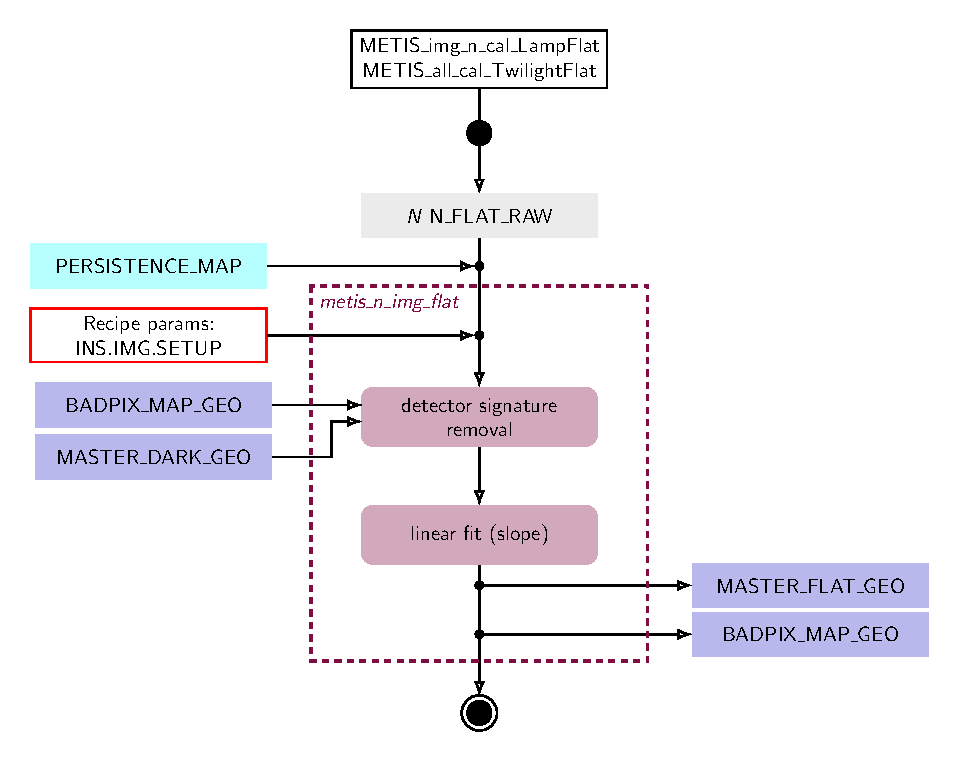
\includegraphics[width=0.6\textwidth]{metis_n_img_flat}
  \caption[Recipe: \REC{metis_n_img_flat}]{\REC{metis_n_img_flat} --
    creation of \CODE{IMG_N} master flatfield}
  \label{fig:metis_n_img_flat}
\end{figure}

%%%%%%%

\subsubsection{N-band imaging chop-nod combination}
\label{img_n_chopnod}
\label{rec:img_n_chopnod}
\label{rec:metis_n_img_chopnod}
\label{sssec:img_n_chopnod}

This recipe combines a set of exposures taken at all positions of a
defined chop-nod pattern and adds/subtracts them into a single
chop/nod difference image. Depending on the actual chop-nod pattern,
this image will contain one or more positive and negative beams.

If flat fielding proves feasible and useful for the GeoSnap detector
the master flat can be applied. If no jitter is applied, i.e.\ if the
beam is at the same detector position for all exposures taken at a
given chop position, then the master flat can be divided into the
final chop-nod difference image. Otherwise, the master flat will have
to be divided into the chop half-cycle images before the jitter
correction is applied.

This fulfills \REQ{METIS-6094}.

\begin{recipedef}
  Name:              & \REC{metis_n_img_chopnod}                                    \\
  Purpose:           & chop/nod combination of exposures for background subtraction \\
  Type:              & Calibration, Science                                         \\
 Templates:          & \TPL{METIS_img_n_cal_standard}                              \\
                     & \TPL{METIS_img_n_obs_AutoChopNod}                            \\
                     & \TPL{METIS_img_n_obs_GenericChopNod}                         \\
                     & \TPL{METIS_img_n_cvc_obs_AutoChop}                           \\
%                     & \TPL{METIS_img_n_clc_obs_FixedSkyOffset}                     \\
                     & \TPL{METIS_img_n_cal_psf}                                    \\
  Input data:        & Chopped/nodded science or standard images                    \\
                     & Bad-pixel map                                                \\
  Matched keywords:  & Filter ID                                                    \\
                     & Chop position                                                \\
                     & Nod position                                                 \\
  Parameters:        & TBD                                                          \\
  Algorithm:         & Add/subtract images to subtract background                   \\
  Output data:       & \hyperref[dataitem:n_sci_bkg_subtracted]{\PROD{N_SCI_BKG_SUBTRACTED}}                                  \\
                     & \hyperref[dataitem:n_std_bkg_subtracted]{\PROD{N_STD_BKG_SUBTRACTED}}                                  \\
  QC1 parameters:    & \QC{N IMG PEAK CNTS}                                         \\
  hdrl functions:    & \CODE{hdrl_imagelist_collapse}                               \\
\end{recipedef}

\begin{figure}[hb]
  \centering
   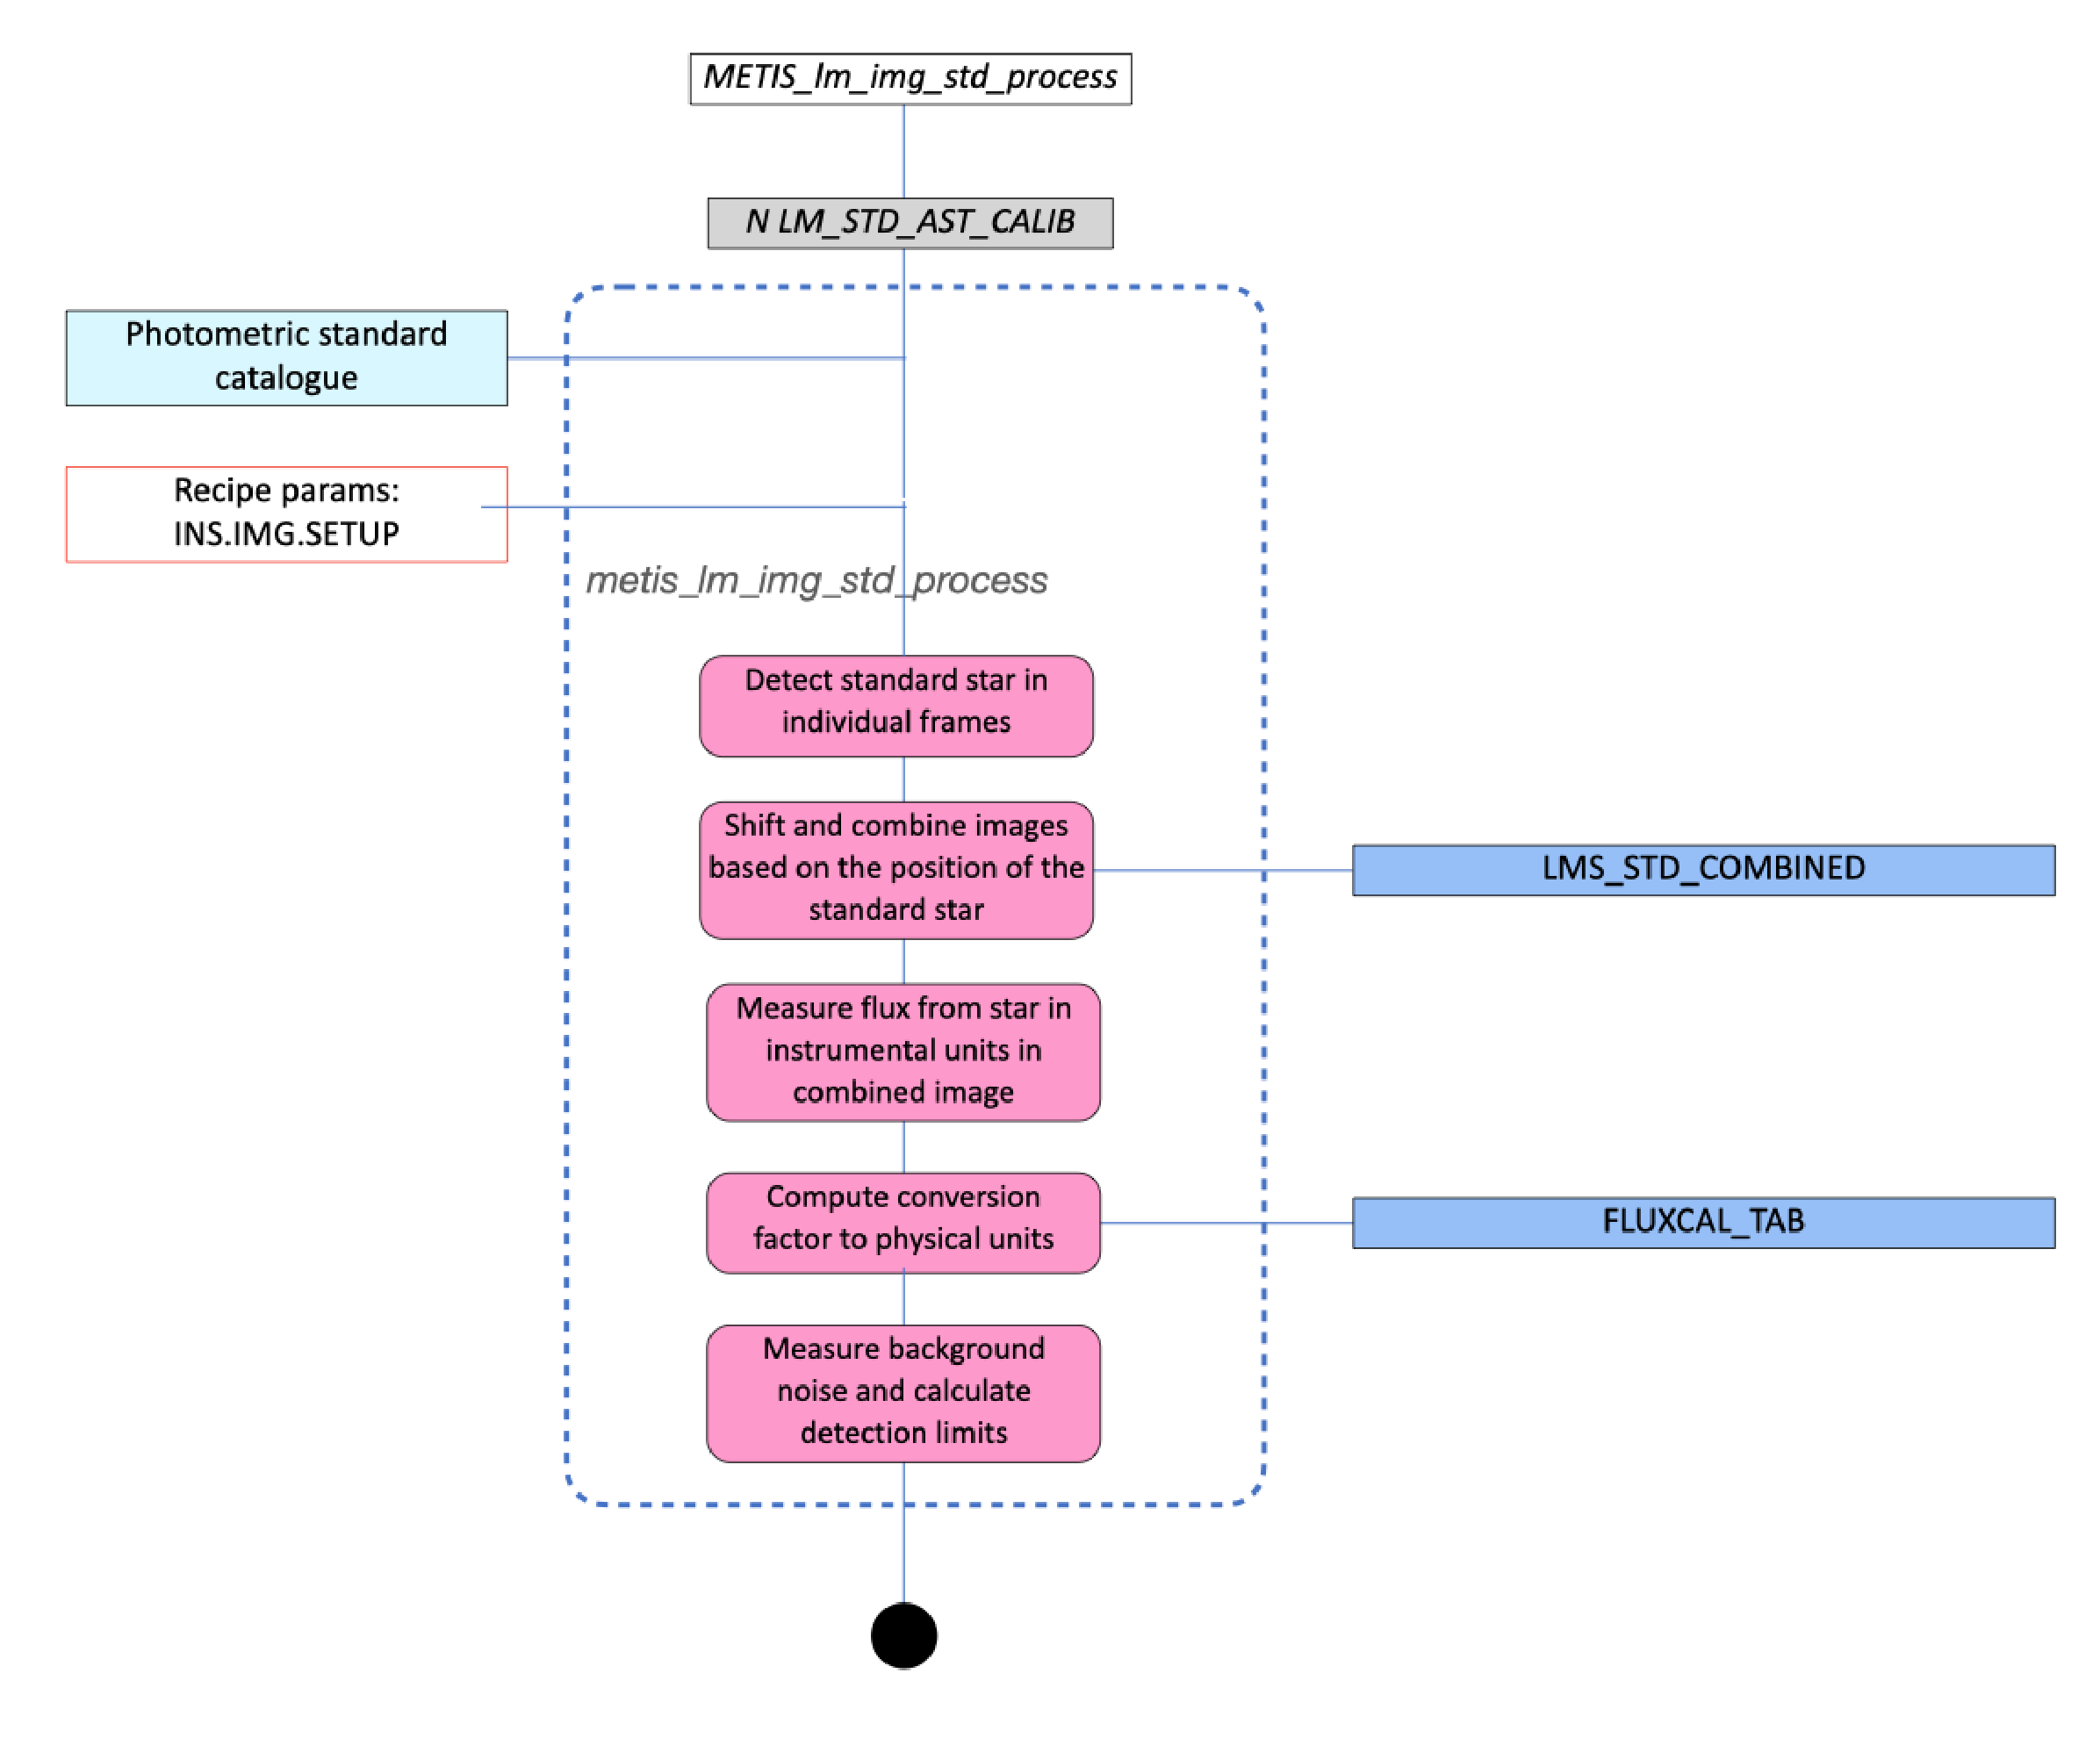
\includegraphics[width=0.6\textwidth]{metis_lm_img_std_process}
  \resizebox{0.6\textwidth}{0.1\textwidth}{\TODO{\fbox{Figure to be done}}}
  \caption[Recipe: \REC{metis_n_img_chopnod}]{\REC{metis_n_img_chopnod} --
    Combination of chop/nodded images.}
  \label{fig:metis_n_img_chopnod}
\end{figure}

%%%%%%%%%%%%%%%%%%%
\clearpage
\subsubsection{N-band imaging photometric standard analysis}
\label{n_img_std_process}
\label{rec:n_img_std_process}
\label{ssec:n_img_std_process}
\label{sssec:n_img_std_process}
\label{metis_n_img_std_process}
\label{rec:metis_n_img_std_process}
\label{sssec:metis_n_img_std_process}

This recipe determines the conversion from ADU to physical units from
a chop-nod difference image of a photometric standard star.  The flux
of the standard star is measured in each of the beams of the chop-nod
difference image, averaged and normalised to an exposure time of
1~second. Comparison to the tabulated brightness of the star in the
observing filter yields the conversion factor from
$\mathrm{ADU}\,\mathrm{s}^{-1}$ to
$\mathrm{photons}\,\mathrm{s}^{-1}\,\mathrm{cm}^{-2}$.

QC parameters will include estimates of the sensitivity for the
detection of point sources and surface brightness sensitivity
following \cite{visir_manual}.

\begin{recipedef}
  Name:                & \REC{metis_n_img_std_process}                                                 \\
  Purpose:             & Determine conversion factor between detector counts and physical source flux. \\
  Type:                & Calibration                                                                   \\
  Templates:           & \TPL{METIS_img_n_cal_standard}                                                \\
  Input data:          & \hyperref[dataitem:n_std_bkg_subtracted]{\PROD{N_STD_BKG_SUBTRACTED}}                                                   \\
                       & photometric standard catalogue                                                \\
  Matched keywords:    & Object ID                                                                     \\
                       & Filter ID                                                                     \\
  Parameters:          & None (TBD)                                                                    \\
  Algorithm:           & call \CODE{n_calculate_std_flux} to measure the flux in all beams\\
                       & average and normalize flux values \\
                       & call \CODE{calculate_std_fluxcal} to calculate conversion factor to physical units   \\
                       & call \CODE{calculate_detection_limits} to compute measured background noise (std, rms) and compute detection limits \\
  Output data:         & \hyperref[dataitem:fluxcal_tab]{\PROD{FLUXCAL_TAB}}                                                            \\
  Expected accuracies: & \TBD                                                                          \\
  QC1 parameters:      & \QC{QC N STD PEAK CNTS}                                                       \\
                       & \QC{QC N STD APERTURE CNTS}                                                   \\
                       & \QC{QC N STD STREHL}                                                          \\
                       & \QC{QC N STD FLUXCONV}                                                        \\
                       & \QC{QC N STD AIRMASS}                                                         \\
                       & \QC{QC N SENSITIVITY}                                                         \\
                       & \QC{QC N AREA SENSITIVITY}                                                    \\
  hdrl functions:      & \CODE{hdrl_catalogue_create}                                                  \\
                       & \CODE{hdrl_strehl_compute}                                                    \\
\end{recipedef}

\begin{figure}[hb]
  \centering
   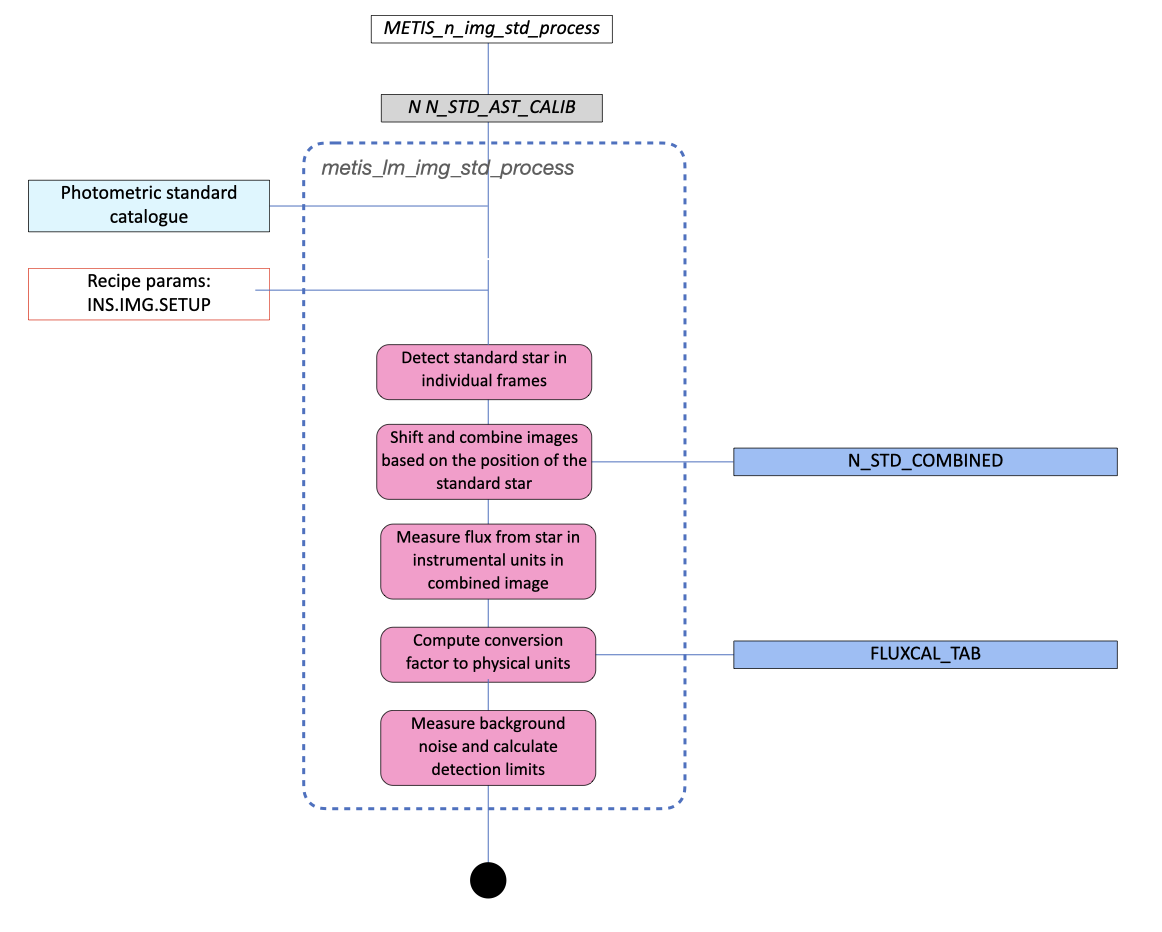
\includegraphics[width=0.6\textwidth]{metis_n_img_std_process}
  %\resizebox{0.6\textwidth}{0.1\textwidth}{\TODO{\fbox{Figure to be done}}}
  \caption[Recipe: \REC{metis_n_img_std_process}]{\REC{metis_n_img_std_process} --
    compute conversion between ADU and physical flux units.}
  \label{fig:metis_n_img_std_process}
\end{figure}


%%%%%%%%%%%%%%%%%%%%%
\clearpage

\subsubsection{N-band imaging calibration}
\label{n_img_calibrate}
\label{rec:n_img_calibrate}
\label{sssec:n_img_calibrate}
\label{rec:metis_n_img_calibrate}

This recipe applies the flux calibration to the chop-nod difference
image. A unique geometric calibration is not possible at this point,
although one could take one of the beams (e.g.\ the positive beam in a
parallel two-point chop-nod pattern) as reference for a
WCS. Distortion information can be added without a reference point as
it pertains to the detector/focal plane, not to the field.

The products of this recipe is the fully calibrated chop-nod
difference image.

The image is multiplied by the conversion factor such that pixel
values are in units of photons per second per centimetre squared. The
header receives the keyword \FITS{BUNIT} with value %
\CODE{'photon.s**(-1).cm**(-2)'}.

\begin{recipedef}
  Name:              & \REC{metis_n_img_calibrate}                      \\
  Purpose:           & Convert science image to physical units          \\
                     & Add distortion information                       \\
  Type:              & Calibration                                      \\
  Templates:         &                                                  \\
  Input data:        & \hyperref[dataitem:n_sci_bkg_subtracted]{\PROD{N_SCI_BKG_SUBTRACTED}}                      \\
                     & \hyperref[dataitem:fluxcal_tab]{\PROD{FLUXCAL_TAB}}                               \\
                     & \hyperref[dataitem:n_distortion_table]{\PROD{N_DISTORTION_TABLE}}                        \\
  Matched keywords:  & Filter ID                                        \\
  Parameters:        & TBD                                              \\
  Algorithm:         & call \REC{n_scale_image_flux} to Scale image data to ph/s \\
                     & call \REC{n_add_header_distortion} to add header information (\FITS{BUNIT}, etc.)\\
  Output data:       & \hyperref[dataitem:n_sci_calibrated]{\PROD{N_SCI_CALIBRATED}}                          \\
  QC1 parameters:    & None                                             \\
\end{recipedef}

\begin{figure}[hb]
  \centering
   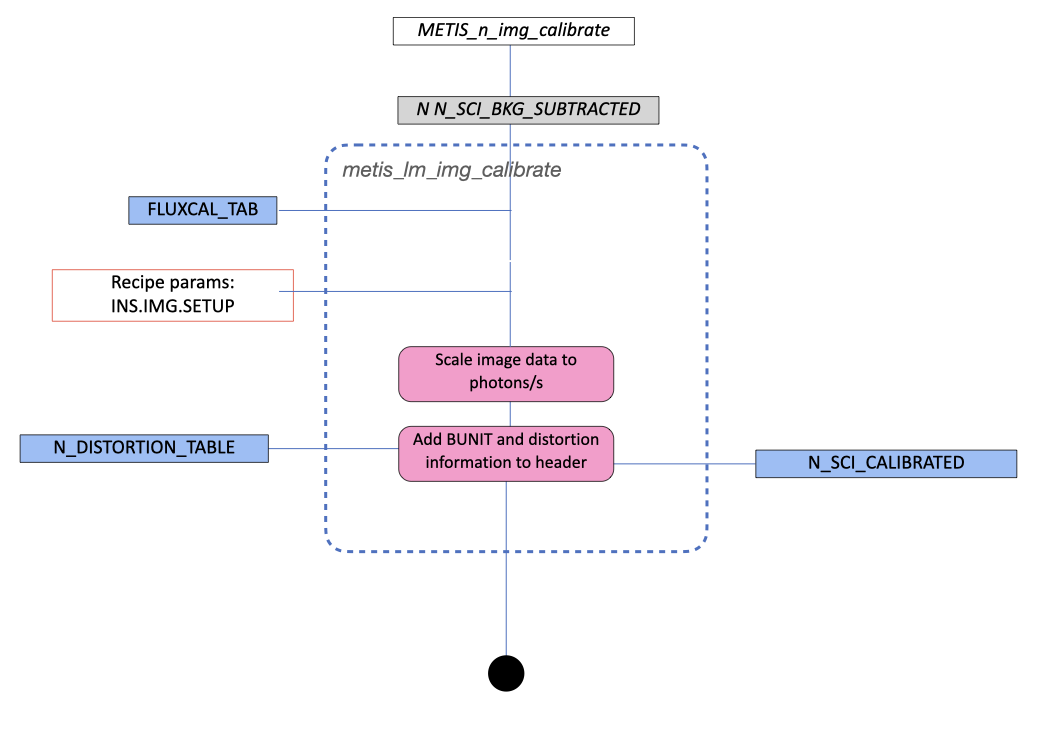
\includegraphics[width=0.6\textwidth]{metis_n_img_calibrate}
  \caption[Recipe: \REC{metis_n_img_calibrate}]{\REC{metis_n_img_calibrate} --
    convert image to physical flux units and update FITS header}
  \label{fig:metis_n_img_calibrate}
\end{figure}

%%%%%%%%%%%%%
\clearpage

\subsubsection{N-band imaging restoration}
\label{n_img_restoration}
\label{rec:n_img_restoration}
\label{sssec:n_img_restoration}

This recipe attempts to combine the positive and negative beams of the
chop-nod difference image into a single positive image of the
source. For compact sources with a size smaller than half the distance
between the beams, it suffices to cut out small regions around the
source images and add the with the appropriate signs to obtain a
single image.

Algorithms for image restoration of extended sources exist but it
remains \TBD\ whether these are sufficiently simple and robust to be
included in the pipeline (cf.\ Sect.~8.8 of \cite{DRLS}).

\begin{recipedef}
  Name:              & \REC{metis_n_img_restore}                                     \\
  Purpose:           & Restore a single positive beam from chop-nod difference image \\
  Type:              & Science                                                       \\
  Input data:        & \hyperref[dataitem:n_sci_calibrated]{\PROD{N_SCI_CALIBRATED}}                                       \\
  Parameters:        & size of cutout region                                         \\
  Algorithm:         & Cut regions around beams                                      \\
                     & Add regions with appropriate signs                            \\
  Output data:       & \hyperref[dataitem:n_sci_restored]{\PROD{N_SCI_RESTORED}}                                         \\
  QC1 parameters:    & None                                                          \\
  hdrl functions:    & \CODE{hdrl_imagelist_collapse}                                \\
\end{recipedef}

\begin{figure}[hb]
  \centering
  % 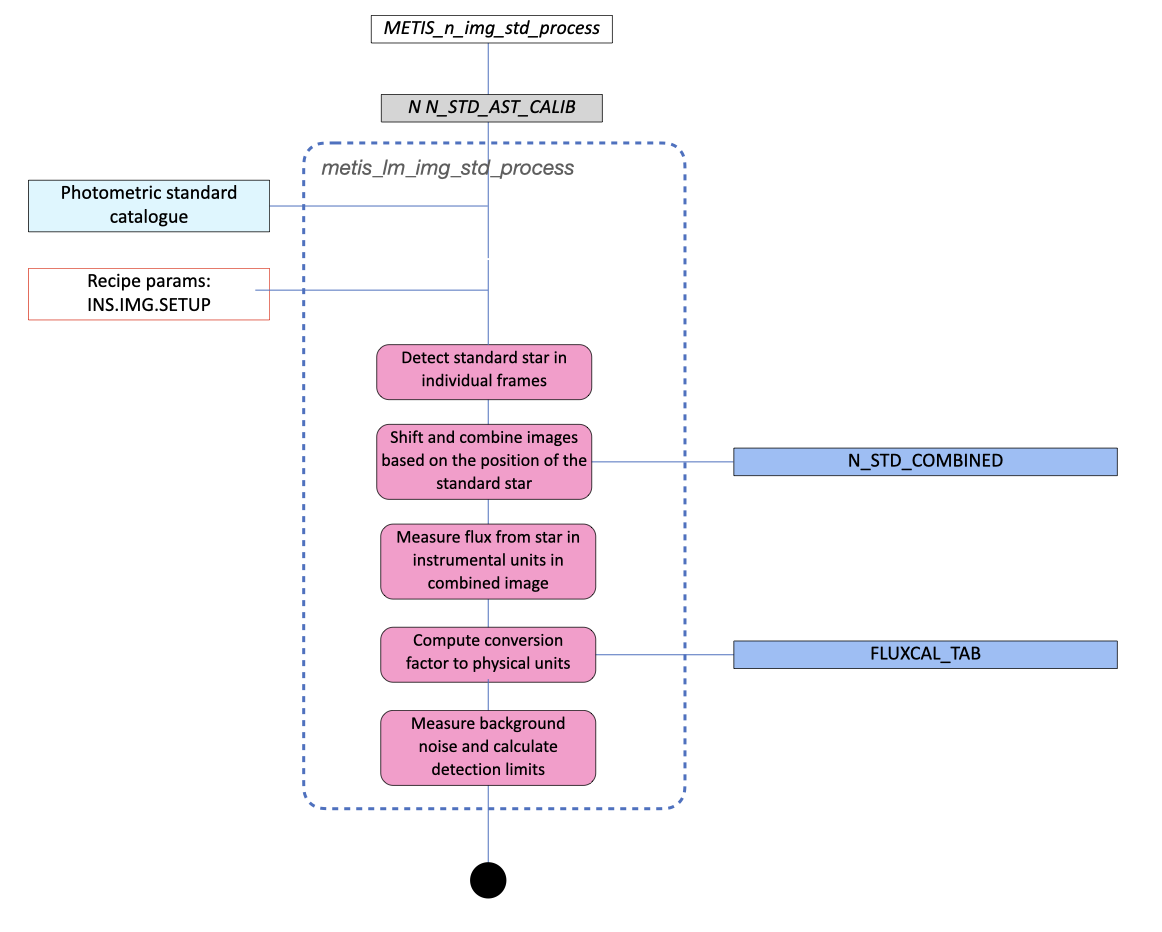
\includegraphics[width=0.6\textwidth]{metis_n_img_std_process}
  \resizebox{0.6\textwidth}{0.1\textwidth}{\TODO{\fbox{Figure to be done}}}
  \caption[Recipe: \REC{metis_n_img_restore}]{\REC{metis_n_img_restore} --
    Create a single positive image from chop-nod difference image}
  \label{fig:metis_n_img_restore}
\end{figure}

%%%%%%%%%%%%%%
\clearpage
\subsubsection{N-band imaging distortion calibration}
\label{rec:metis_n_img_distortion}
\label{n_img_distortion}
\label{rec:n_img_distortion}
\label{sssec:n_img_distortion}

Calibration of the imaging distortion is done on an image of a pin
hole mask located in a focal plane within the instrument. The
distortion is described in terms of a polynomial model whose
coefficients can be transformed to WCS keywords and applied to any
other pipeline product. In addition to the distortion table, a map of
pixel scale across the detector will be created.

\begin{recipedef}
  Name:                & \REC{metis_n_img_distortion}                                   \\
  Purpose:             & Determine optical distortion coefficients for the N imager.    \\
  Templates:           & \TPL{METIS_img_n_cal_distortion}                               \\
  Type:                & Calibration                                                    \\
  Input data:          & Images of grid mask in WCU-FP2 or CFO-FP2.                     \\
                       & Image with WCU window closed (background).                     \\
                       & Grid of pinhole mask positions \\
                       & Bad pixel map                                                  \\
  Parameters:          & Parameters for fitting routine \\
                       & \TBD \\
  Algorithm:           & Subtract background image.  (\CODE{hdrl_imagelist_sub_image})                                       \\
                       & Measure location of point source images in frames.   (\CODE{hdrl_catalogue_create})            \\
                       & call \hyperref[drl:fit_distortion]{\CODE{fit_distortion}} to fit polynomial coefficients to deviations from grid positions. \\
  Output data:         & \hyperref[dataitem:n_distortion_table]{\PROD{N_DISTORTION_TABLE}} \\
                       & \hyperref[dataitem:n_distortion_map]{\PROD{N_DISTORTION_MAP}}        \\
                       & \hyperref[dataitem:n_dist_reduced]{\PROD{N_DIST_REDUCED}}             \\
  Expected accuracies: & TBD                                                            \\
  QC1 parameters:      & \hyperref[qc:qc_n_distort_rms]{\QC{QC N DISTORT RMS} }                                         \\
                       & \hyperref[qc:qc_n_distort_nsource]{\QC{QC LM DISTORT NSOURCE}}  \\
  hdrl functions:      & \CODE{hdrl_catalogue_create}                                   \\
                       & \CODE{hdrl_imagelist_sub_image}                                \\
\end{recipedef}

\begin{figure}[hb]
  \centering
  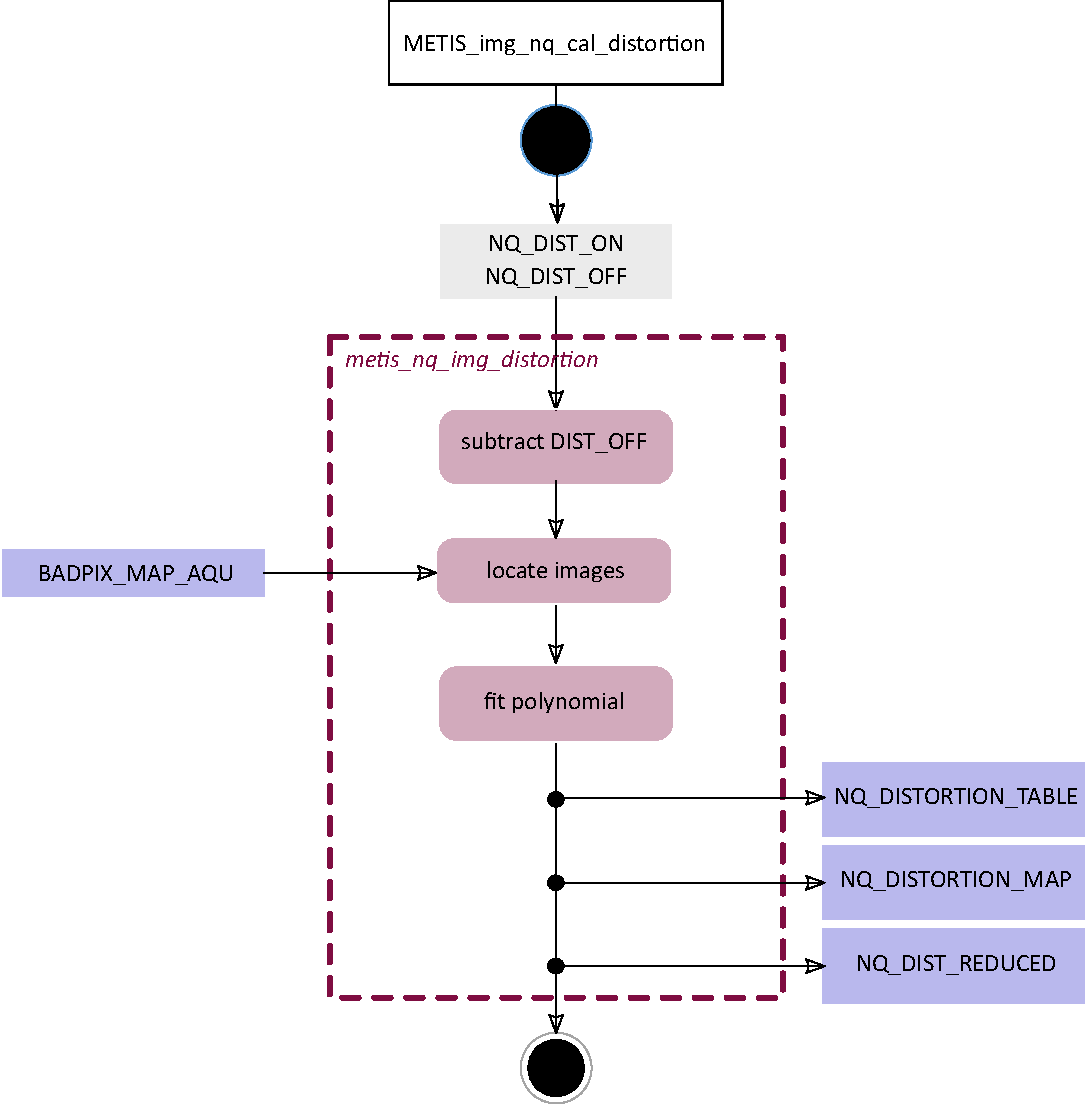
\includegraphics[width=0.6\textwidth]{metis_n_img_distortion}
  \caption[Recipe: \REC{metis_n_img_distortion}]{%
    \REC{metis_n_img_distortion} -- \CODE{IMG_N} distortion calibration}
  \label{fig:metis_n_img_distortion}
\end{figure}

%%% Local Variables:
%%% TeX-master: "METIS_DRLD"
%%% End:
